\documentclass[conference]{IEEEtran}
\IEEEoverridecommandlockouts
% The preceding line is only needed to identify funding in the first footnote. If that is unneeded, please comment it out.
\usepackage[english,brazil]{babel}
\usepackage{cite}
\usepackage{amsmath,amssymb,amsfonts}
\usepackage{algorithmic}
\usepackage{graphicx}
\usepackage{textcomp}
\usepackage{xcolor}
\usepackage[show]{ed}

%comandos para o meu comentário
\newcommand{\xexeo}[1]{\ednote{\textcolor{red}{Xexéo - #1}}}
\newcommand{\carla}[1]{\ednote{\textcolor{purple}{Carla - #1}}}
\newcommand{\julio}[1]{\ednote{\textcolor{blue}{Júlio - #1}}}
\newcommand{\horacio}[1]{\ednote{\textcolor{navy}{Horácio - #1}}}

\def\BibTeX{{\rm B\kern-.05em{\sc i\kern-.025em b}\kern-.08em
    T\kern-.1667em\lower.7ex\hbox{E}\kern-.125emX}}
    
\begin{document}

\title{Léo \& Maya: um jogo para auxiliar no ensino de pensamento computacional
}

\author{
\IEEEauthorblockN{[AVALIAÇÃO CEGA]}
\IEEEauthorblockA{[AVALIAÇÃO CEGA]}
}

%\author{
\IEEEauthorblockN{Horácio B. M. Henriques}
\IEEEauthorblockA{\textit{Instituto de Computação} \\\textit{Universidade Federal do Rio de Janeiro}\\Rio de Janeiro, Brasil \\horacio97@dcc.ufrj.br}\\
\IEEEauthorblockN{Carla A. D. M. Delgado}
\IEEEauthorblockA{\textit{Instituto de Computação} \\\textit{Universidade Federal do Rio de Janeiro} \\Rio de Janeiro, Brasil \\carla@dcc.ufrj.br}\\
\and
\IEEEauthorblockN{Júlio R. K. Mandoju}
\IEEEauthorblockA{\textit{Instituto de Computação} \\\textit{Universidade Federal do Rio de Janeiro} \\Rio de Janeiro, Brasil \\juliorkm@dcc.ufrj.br} \\
\IEEEauthorblockN{Geraldo Xexéo}
\IEEEauthorblockA{\textit{Prog. de Engenharia e Sistemas de Informação} \\\textit{COPPE}\\\textit{Instituto de Computação}\\\textit{Universidade Federal do Rio de Janeiro}\\Rio de Janeiro, Brasil \\gxexeo@cos.ufrj.br}
}

\maketitle

\selectlanguage{brazil}
\begin{abstract}
Em um mundo com cada vez mais computadores, é imprescindível que as pessoas saibam resolver problemas usando computadores de forma eficaz. Para tal, é necessário introduzir pessoas ao pensamento computacional: um meio de resolver problemas que consiste em interpretar e dividir problemas grandes em problemas menores com soluções conhecidas e descrever essa solução na forma de um algoritmo. O jogo Léo \& Maya é uma forma de ajudar no ensino de pensamento computacional para crianças de sete a onze anos. Ele consiste em vinte e duas fases de complexidade crescente onde o jogador é levado a montar algoritmos usando um conjunto específico de instruções para completar objetivos específicos, por vezes fazendo uso de pensamento computacional paralelo para controlar mais de um personagem dentro de uma fase. Apesar da validação ter ocorrido durante a pandemia do Covid-19, que limitou o acesso aos voluntários entrevistados, a recepção por parte dos professores entrevistados, responsáveis por alunos dentro da faixa etária pretendida foi positiva, apontando para um futuro promissor para o projeto.
\end{abstract}

\renewcommand{\IEEEkeywordsname}{Palavras-Chave}
\begin{IEEEkeywords}
pensamento computacional, pensamento computacional paralelo, jogos educativos.
\end{IEEEkeywords}

\section{Introdução}

Pensamento Computacional (PC) é um assunto que tem ganhado cada vez mais relevância ao longo dos últimos anos em discussões sobre educação infantil \cite{b1}. Citado pela primeira vez por Jeanette Wing em 2006, PC foi vagamente definido como ``resolução de problemas, idealização de sistemas e compreensão do comportamento humano através de conceitos fundamentais à ciência da computação''\cite{b2} e, desde então, se constitui em objeto de discussão no meio acadêmico, da definição até a aplicabilidade em salas de aula.

Hoje em dia, compreende-se que PC seja um conjunto de habilidades necessárias, comumente divididas em quatro técnicas (ou pilares): abstração, decomposição em subproblemas, reconhecimento de padrões e criação de algoritmos\cite{b3}. Essas habilidades seriam úteis não só para um programador que precisa escrever códigos com algum objetivo prático, mas para qualquer pessoa que precise resolver um problema.

Cada vez mais currículos de ensino médio e ensino fundamental estão agregando conteúdos de PC. Por exemplo, o plano de currículo K-12, dos Estados Unidos tem flertado com conceitos de PC desde 2011\cite{b1}, vindo a cada vez mais empregar esforços ao longo de anos para agregar conteúdos de PC no currículo de crianças e adolescentes. Já no Brasil, a Base Nacional Comum Curricular (BNCC) aprovada em dezembro de 2017 menciona explicitamente, na seção de ensino matemático, aplicações de álgebra no desenvolvimento de PC através do uso de algoritmos como estratégia para resolver problemas matemáticos\cite{b4}.

Currículos escolares normalmente não abordam o assunto de pensamento computacional paralelo (PCP). Por mais que tenha sido mencionado por Wing em 2006 em seu primeiro artigo seminal sobre o assunto, e mais uma vez destrinchado em maior detalhe por Kirkpatrick no artigo "Parallel Computer Thinking" em 2017, PCP é tido como um assunto que pode ser complexo demais para um aluno ter tempo de aprender em sala de aula, apesar de sua importância\cite{b5}. 

De modo a auxiliar o ensino de PC para jogadores em idade escolar,  foi desenvolvido o jogo educativo endógeno Léo e Maya.  O objetivo é ensinar, através de uma abordagem lúdica, como fazer uso de PC para a resolução de problemas que admitem soluções algorítmicas, contemplando também o ensino de PCP. Os ensinamentos serão passados através de várias fases onde os jogadores montarão algoritmos que serão seguidos pelos personagens do jogo — o gato Léo e a cachorra Maya — de modo a solucionar o problema proposto pela fase.

\section{Fundamentação Teórica}

\subsection{Pensamento Computacional e Pensamento Computacional Paralelo}

Pensamento computacional (PC) é mais do que meramente saber pensar para programar. PC envolve resolver subproblemas, desenhar sistemas e compreender comportamento humano ao se utilizar de conceitos fundamentais à ciência da computação\cite{b2}. É uma síntese de formas de pensar que são normalmente divididas em quatro pilares fundamentais: a decomposição de problemas, o reconhecimento de padrões, a abstração de informações e a formulação de algoritmos\cite{b6}.

 Essa forma de pensamento e resolução não é útil somente ao programador, mas também para qualquer pessoa. PC influencia outros campos de estudo, como ``medicina algorítmica, arqueologia computacional, economia computacional, finanças computacionais, computação e jornalismo, direito computacional, ciências sociais computacionais e humanidades digitais\cite{b7}''. E mesmo fora destes campos de estudo, PC é útil uma vez que dá às pessoas a capacidade de adaptar soluções algorítmicas, avaliar quando um computador é melhor indicado para lidar com um problema e aplicar estratégias como divisão e conquista na resolução de problemas na vida cotidiana\cite{b7}.

PC é uma habilidade comumente relacionada com currículos de computação\cite{b8} ou matemática, uma vez que os alunos precisam ``ser capazes de traduzir uma situação dada em outras linguagens, como transformar situações-problema, apresentadas em língua materna, em fórmulas, tabelas e gráficos e vice-versa''\cite{b4} para a aprendizagem de álgebra e outros campos da matemática. 

A discussão sobre o ensino de PC não é atual, tendo em vista que ações para o ensino de computação à crianças, como por exemplo o uso de LOGO ou de Basic para fins didáticos, são discutidas desde os anos 80\cite{b9}. Contudo, a atenção ao assunto cresceu quando, em 2006, Wing definiu em seu artigo ``Computational Thinking'' o que é PC e estabeleceu a importância dessa prática. Desde então, trabalhos têm sido produzidos de modo a explorar formas de integrar o ensino de PC em turmas de ensino fundamental e médio\cite{b1}\cite{b10}\cite{b11}\cite{b12}.

Contudo, no mundo de hoje, pessoas têm acesso a computadores, smartphones e tablets com multiprocessadores, permitindo que todo tipo de aplicação execute tarefas em paralelo, algo que não era possível até aproximadamente uma década atrás, quando a computação paralela se tornou convencional.  Portanto, é importante que se contemple também o ensino de pensamento computacional paralelo (PCP),  que traz consigo muitas vantagens\cite{b5}.

Um dos benefícios da computação paralela é que ela ``ajuda a desenvolver uma abordagem mais flexível para solucionar problemas porque há mais modelos nos quais se basear.''\cite{b5} Além disso, o paralelismo oferece mais formas de quebrar um problema grande em subproblemas menores, algo que pode acrescentar às vantagens de se aprender o pensamento computacional, considerando que a decomposição de problemas é um de seus pilares fundamentais\cite{b5}.

\subsection{Jogos Educativos Endógenos}

Quando se discutem jogos educativos, é importante levar em conta como o conteúdo pedagógico a ser ensinado para o jogador está integrado no jogo, uma vez que o sucesso do jogo como atividade didática depende do quão intrínsecos são os conteúdos abordados dentro da fantasia oferecida pelo jogo \cite{b13}. Nisso, podemos aqui ver a divisão de jogos educativos em duas categorias: os jogos educativos sendo exógenos ou endógenos\cite{b14}.

O jogo educativo exógeno é, por natureza, mais fácil de ser feito e executado, e por isso tem tido maior adoção por professores.\cite{b14} A característica mais marcante desse tipo de jogo educativo é o destacamento das regras do jogo para com o conteúdo que se quer ensinar.  Um exemplo desse tipo de jogo seriam perguntas-e-respostas, onde as regras do jogo independem do conteúdo das perguntas e meramente coexistem com o conteúdo.

Por outro lado, o jogo educativo endógeno possui necessariamente uma ligação entre o \textit{game design} e o conteúdo a ser passado. Sua maior característica é fazer com que o domínio do jogo venha agregado ao domínio do próprio conteúdo, como por exemplo em jogos de estratégia históricos como as séries Civilization e Rise of Nations\cite{b14}.

\subsection{Jogos "de programação"}

Em lojas virtuais de jogos, uma categoria presente de jogos são \textit{puzzle games} sobre programar soluções em ambientes simulados\cite{b15}\cite{b16}, vindo a serem categorizados como ``\textit{programming games}'' dependendo da plataforma\cite{b17}. A existência de outros jogos que abordam temas similares a Léo \& Maya é excelente, uma vez que prova a existência de um mercado para esse tipo de jogo e informa uma coleção de convenções e ideias sobre as quais o nosso jogo pode construir.

Todos os jogos contemplados dentro dessas categorias funcionam de forma suficientemente similar. Normalmente, eles são divididos em fases, e cada fase dá um problema a ser resolvido para o qual o jogador declara um algoritmo que solucione o problema proposto, cada jogo propondo uma forma de declaração de instrução diferente.

Um exemplo de jogo que se encaixa nesta categoria é o Human Resource Machine\cite{b18}, um jogo que ensina lógica de programação através de várias fases onde o jogador escreve algoritmos enfileirando blocos que significam instruções simples que lembram \textit{Assembly} de modo a concluir objetivos. Human Resource Machine serviu de inspiração não só como prova de que esse tipo de jogo era viável e tem um público, mas também como prova de que jogos sobre montar algoritmos eram possíveis em celulares.

\section{Projeto do Jogo Educativo}
Antes do desenvolvimento do jogo, criou-se um \textit{game design canvas} baseado no Game Design Canvas para jogos endógenos (Endo-GDC) de modo a ``facilitar a discussão e descrição de um jogo sério''\cite{b19}. O canvas é útil para unificar a linguagem usada por todas as partes envolvidas na produção do \textit{game} e descrever de forma explícita e legível a relação entre o conteúdo que se quer passar, os objetivos pedagógicos que querem ser atingidos através do conteúdo e as mecânicas do jogo que deverão ter ligação direta com os objetivos. Todo o conteúdo desse canvas foi, num momento posterior, traduzido em um documento de\textit{game design}.

No que diz respeito aos aspectos técnicos, utilizou-se a Unity\cite{b20} para construir o jogo. A Unity é um motor de jogos gratuito estabelecido no mercado que permite a criação de aplicações com recursos gráficos tanto em 2D quanto 3D, e que possui um foco no mercado de desenvolvimento de jogos eletrônicos. Atualmente, a Unity utiliza C\#\cite{b21} como a linguagem para escrever \textit{scripts} dentro dos projetos, e permite a exportação dos seus projetos para, dentre outras plataformas, computadores pessoais e celulares Android. Contudo, toda a arte do jogo foi produzida usando o aplicativo pago Aseprite\cite{b22}.

O conteúdo pedagógico que o jogo visa abordar está alinhado com currículos de cursos de programação ao redor do mundo\cite{b8}\cite{b23}, introduzindo conteúdos pontuais desses mesmos currículos na ordem em que eles aparecem nos planos de aulas. A diferença é a introdução de paralelismo por parte do jogo, conteúdo que não aparece em nenhum dos currículos consultados. Através dos conteúdos pedagógicos, o jogo visa exercitar a construção de algoritmos e a divisão de problemas complexos em subproblemas simples de solução conhecida, dois dos quatro pilares fundamentais de PC\cite{b6}.

O jogo possui um total de vinte e duas fases divididas em seis seções que introduzem mecânicas e conteúdos diferentes. As fases do jogo funcionam todas praticamente da mesma forma, de modo a manter a consistência na interação do jogador com as mecânicas do jogo e não exigir que o jogador reaprenda a jogar a cada fase. Caso a fase seja a primeira de algum conjunto de fases e o jogador estiver jogando a fase pela primeira vez, um vídeo demonstra através de um exemplo a mecânica nova que o conjunto de fases introduz.

Independente de qual for a fase dentro do seu grupo de fases, todas as fases se dão como descrito a seguir. O jogador tem acesso à visão inteira do mapa da fase, a uma descrição do objetivo e todo o tempo do mundo para conceber uma resposta. Contudo, desde o início da fase, o jogador é livre para arrastar instruções, representadas por artefatos visuais, até a trilha de instruções localizada no canto da tela.

\begin{figure}[htbp]
\centerline{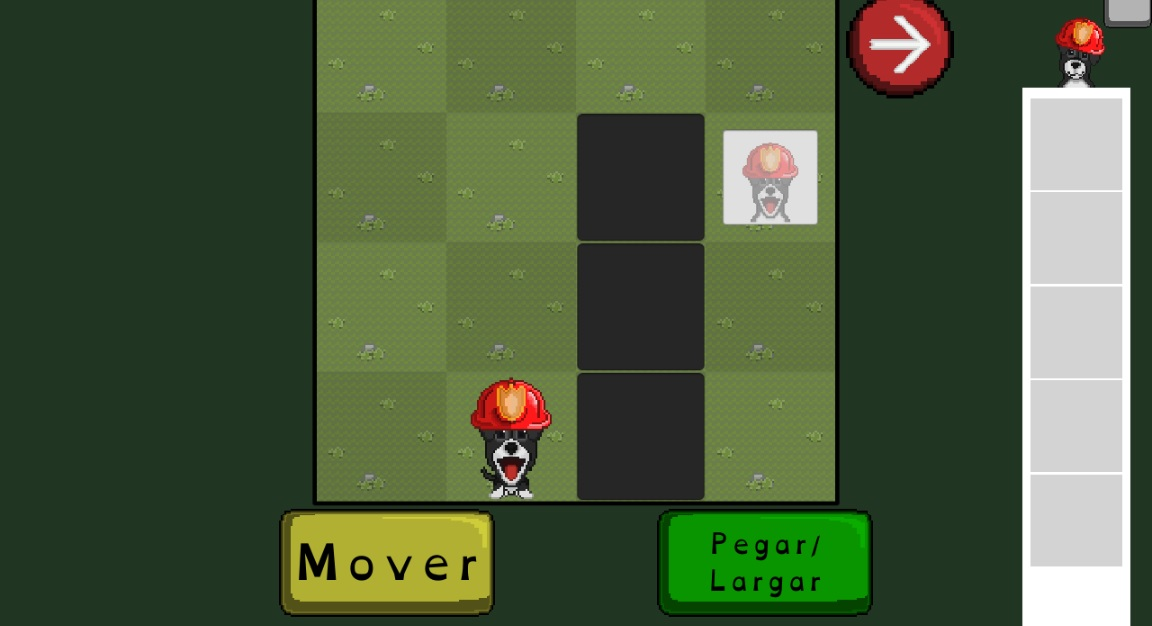
\includegraphics[scale=0.275]{images/fig01.jpg}}
\caption{Início da fase 5-1, a primeira fase que aborda laços de instruções.}
\label{fig}
\end{figure}

Assim que o jogador se der por satisfeito com a solução concebida, o jogador deve apertar no botão ``pronto'' presente na figura acima para dar continuidade. Se o jogo não tiver sido introduzido a laços de instruções, o jogador será levado diretamente para a execução do algoritmo. Caso contrário, o jogador terá a liberdade de definir laços de instruções com um número finito de repetições. Nesta tela, o jogador também tem toda a liberdade de retornar para a tela anterior e fazer algum ajuste às instruções presentes na trilha e voltar a ela.
\begin{figure}[htbp]
\centerline{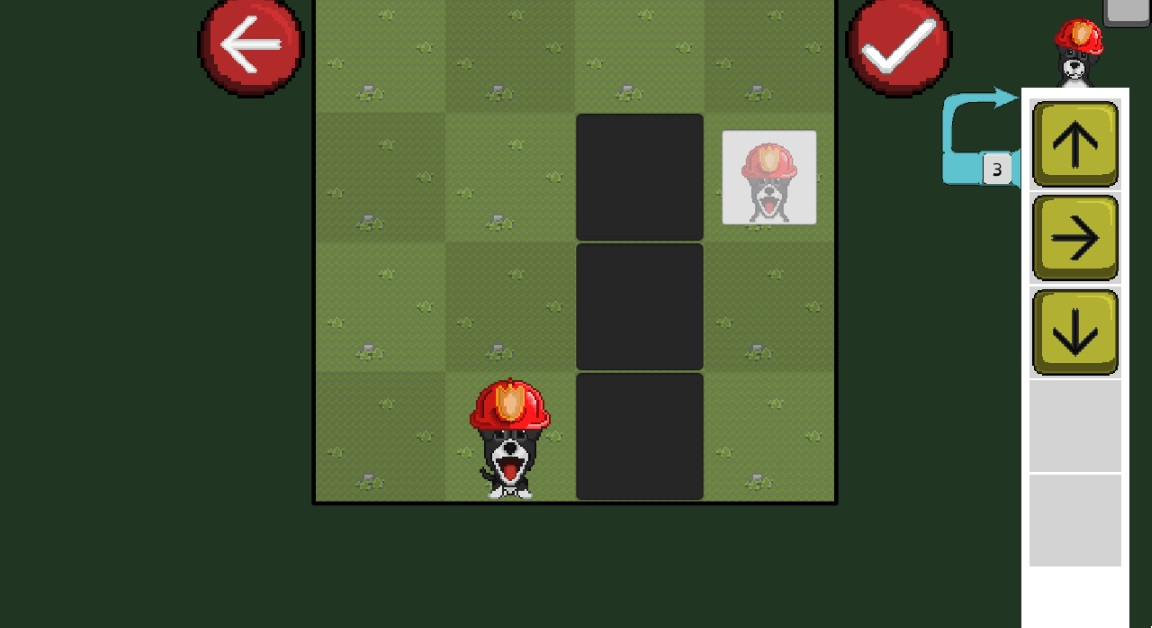
\includegraphics[scale=0.275]{images/fig02.jpg}}
\caption{Tela de declaração de laços de insturções da fase 5-1.}
\label{fig}
\end{figure}

Uma vez que o algoritmo for executado, o jogo rodará por todas as instruções até que um dos dois cenários ocorram: ou o personagem cumpre o objetivo proposto pela fase seguindo o algoritmo concebido pelo jogador, ou o jogador fornecerá ao personagem um algoritmo incapaz de resolver a fase. Em caso de sucesso, o jogador terá a opção de voltar ao menu principal ou jogar a mesma fase novamente, como visto na figura abaixo. Então o jogador poderá voltar ao menu principal e selecionar a próxima fase para jogar. Caso contrário, no lugar da imagem de sucesso, o jogo explicará o que aconteceu de errado na execução do algoritmo e permitirá que o jogador jogue a fase de novo.
\begin{figure}[htbp]
\centerline{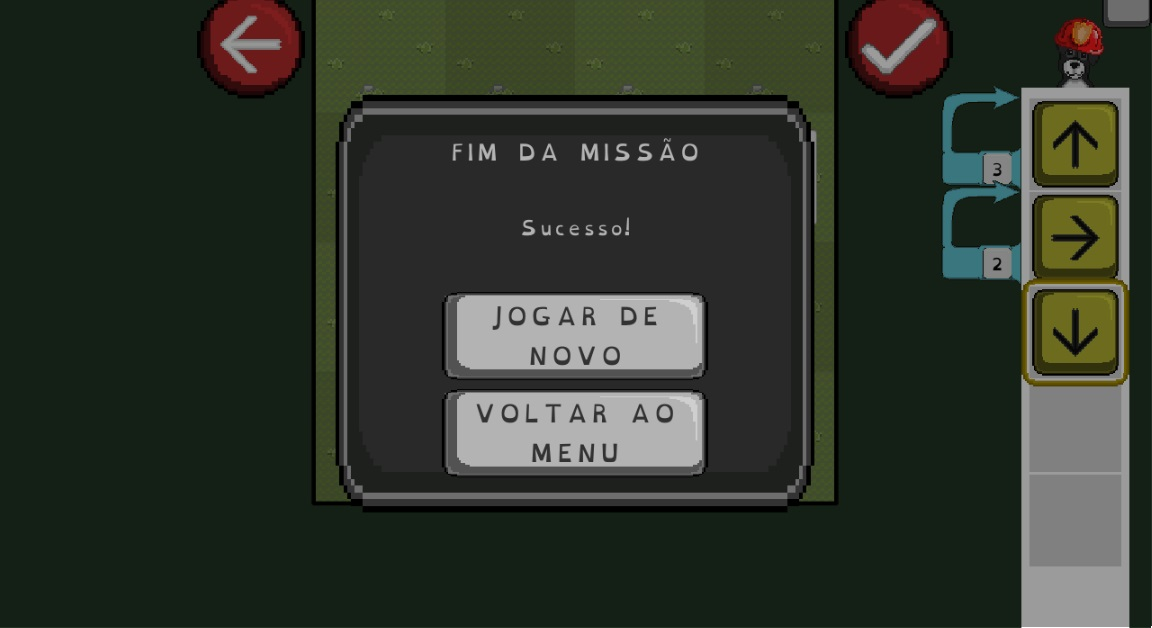
\includegraphics[scale=0.275]{images/fig03.jpg}}
\caption{Tela de sucesso da fase 5-1.}
\label{fig}
\end{figure}

\section{Validação}

A validação do trabalho se deu durante a pandemia do Covid-19, que foi um desafio por si só. Além da pandemia, nosso público-alvo são menores de idade, o que motivou a fazer a validação com professores de diferentes faixas etárias de modo a contemplar a impressão que o jogo pode causar em pessoas de fora da faixa etária pretendida. Desta forma, a validação se deu na forma de uma pesquisa qualitativa onde, através de mensagens eletrônicas por \textit{e-mail} ou \textit{facebook}, professores receberam o link para acessar o jogo, um questionário com uma explicação breve sobre pensamento computacional e cinco páginas com perguntas sobre o histórico do professor acerca do uso de jogos didáticos e a opinião sobre diferentes aspectos do jogo. 

No início da busca por professores voluntários, o foco se restringiu a professores de matemática ou informática, tendo em vista a proximidade dos conteúdos. Contudo, de modo a contemplar pontos de vista de pessoas de fora da área e desta forma fazer de Léo \& Maya mais acessível para indivíduos sem conhecimento prévio sobre pensamento computacional, esse escopo foi expandido para professores de todas as matérias. Ao final da pesquisa, onze voluntários foram contemplados. Destes onze, três deles dão aula para a faixa etária alvo do jogo, enquanto que os outros oito dão aula para alunos mais velhos ou mais novos; e sete deles dão aula de matemática e/ou computação. Um dos professores entrevistados leciona especificamente a matéria "pensamento computacional" para alunos de cinco a sete anos.

A recepção por parte dos voluntários foi positiva. Nenhum voluntário expressou ter desgostado completamente do jogo, apesar de comentários de professores com alunos na idade de ensino médio questionarem a validez do jogo na hora de ensinar algo aos seus alunos, ou se o jogo não seria visto como infantil demais. Um professor específico de ensino médio apontou a falta de um enredo com personagens desenvolvidos como uma falha, uma vez que isso comprometeria o engajamento emocional de jogadores mais velhos. Outros problemas que professores tiveram de modo geral, independente da faixa etária ou matérias, foram com os tutoriais e a falta de \textit{feedback} audiovisual em tempo real ao bater em paredes, o que tornava a mensagem de erro que aparecia confusa, De modo geral, o retorno foi positivo, ainda assim.

\section{Conclusão e Trabalhos Futuros}

Pensamento Computacional é uma habilidade cada vez mais relevante tanto em currículos escolares quanto na vida cotidiana. E recentemente, com a inclusão de PC em currículos escolares, que costumam relacionar esse conteúdo com matérias dedicadas à computação ou algebra, a discussão sobre como exercitar tal habilidade tem tomado maior relevância. Com o objetivo de ajudar no ensino de PC, criou-se Léo \& Maya: um jogo educativo para celulares Android feito em Unity voltado para o público em idade escolar sobre uma cachorra e um gato bombeiros que ajudam animaizinhos em apuros que visa ensinar sobre pensamento computacional sequencial e paralelo. Ao longo de vinte e duas fases, o jogo busca ensinar sobre construção de algoritmos para resolver problemas e reconhecimento de subproblemas dentro de problemas grandes, ao mesmo tempo em que familiariza seu público com o conceito de paralelizar soluções de problemas e lidar com as condições em que isso implica. 

Para o futuro próximo, existe o objetivo de retrabalhar os tutoriais de modo que eles sejam mais acessíveis a um número maior de pessoas na hora de ensinar como jogar o jogo. Também existe a ambição de colocar artifícios de comunidade, como uma forma de criar fases customizáveis e de compartilhar estas mesmas fases e \textit{leaderboards} para estimular competetividade entre jogadores e aperfeiçoamento na hora de montar algoritmos, e implementar uma quantidade maior de arte de modo a fazer o jogo mais sensorialmente agradável de se jogar,


%\section*{Agradecimentos}
%
%The preferred spelling of the word ``acknowledgment'' in America is without 
%an ``e'' after the ``g''. Avoid the stilted expression ``one of us (R. B. 
%G.) thanks $\ldots$''. Instead, try ``R. B. G. thanks$\ldots$''. Put sponsor 
%acknowledgments in the unnumbered footnote on the first page.


\begin{thebibliography}{23}
\bibitem{b1} V. Barr e C. Stephenson, ``Bringing computational thinking to K-12: what is Involved and what is the role of the computer science education community?'', ACM Inroads, vol. 2, nº 1, Art. nº 1, fev. 2011, doi: 10.1145/1929887.1929905.
\bibitem{b2} J. M. Wing, ``Computational Thinking'', Communications of the ACM, vol. 49, nº 3, Art. nº 3, mar. 2006.
\bibitem{b3} C. P. Brackmann, ``Desenvolvimento do Pensamento Computacional Através de Atividades Desplugadas na Educação Básica'', Doutorado, Universidade Federal do Rio Grande do Sul, Porto Alegre, 2017.
\bibitem{b4} M. Filho, ``MINISTRO DE ESTADO DA EDUCAÇÃO'', p. 472.
\bibitem{b5} K. Kirkpatrick, ``Parallel computational thinking'', Commun. ACM, vol. 60, nº 12, Art. nº 12, nov. 2017, doi: 10.1145/3148760.
\bibitem{b6} ``What is computational thinking? - Introduction to computational thinking - KS3 Computer Science Revision'', BBC Bitesize. https://www.bbc.co.uk/bitesize/guides/zp92mp3/revision/1 (acessado abr. 17, 2021).
\bibitem{b7} J. M. Wing, ``Computational Thinking: What and Why?'', Link Magazine, p. 1–6, nov. 2010.
\bibitem{b8} ``TCH060: C++ Programming''. https://www.k12.com/high-school-course-list/cplusplus-programming-elective-tch060.html (acessado jun. 23, 2020).
\bibitem{b9} S. Grover e R. Pea, ``Computational Thinking in K–12: A Review of the State of the Field'', Educational Researcher, vol. 42, nº 1, Art. nº 1, jan. 2013, doi: 10.3102/0013189X12463051.
\bibitem{b10} R. S. de França, Ferreira Victor Afonso dos Santos Ferreira, L. C. F. de Almeida, e H. J. C. do Amaral, ``A disseminação do pensamento computacional na educação básica: lições aprendidas com experiências de licenciandos em computação'', p. 10, 2014.
\bibitem{b11} A. Repenning, A. Basawapatna, e N. Escherle, ``Computational thinking tools'', in 2016 IEEE Symposium on Visual Languages and Human-Centric Computing (VL/HCC), Cambridge, United Kingdom, set. 2016, p. 218–222, doi: 10.1109/VLHCC.2016.7739688.
\bibitem{b12} R. Monclar, ``Jogos com Propósito para o Ensino de Programação'', p. 9.
\bibitem{b13} M. P. J. Habgood, S. E. Ainsworth, e S. Benford, ``Endogenous fantasy and learning in digital games'', Simulation \& Gaming, vol. 36, nº 4, p. 483–498, dez. 2005, doi:10.1177/1046878105282276.
\bibitem{b14} R. Halverson, ``What Can K-12 School Leaders Learn from Video Games and Gaming?'', p. 8.
\bibitem{b15} ``Google Play''. https://play.google.com/store/apps/category/\linebreak GAME\_PUZZLE (acessado abr. 17, 2021).
\bibitem{b16} ``GOG.com'', GOG.com. www.gog.com (acessado abr. 17, 2021).
\bibitem{b17} ``Produtos com marcador ‘Programação’''. https://store.steampowered.com/tags/pt-br/Programa\%C3\%A7\%C3\%A3o/ (acessado abr. 17, 2021).
\bibitem{b18} ``Human Resource Machine – Apps no Google Play''. https://play.google.com/store/apps/details?id=com.tomorrowcorporation.\linebreak humanresourcemachine\&hl=pt\&gl=BR (acessado abr. 17, 2021).
\bibitem{b19} B. B. Taucei, ``Endo-GDC: Desenvolvimento de um Game Design Canvas para Jogos Sérios Endógenos'', p. 105.
\bibitem{b20} U. Technologies, ``Unity Real-Time Development Platform | 3D, 2D VR \& AR Engine''. https://unity.com/ (acessado abr. 17, 2021).
\bibitem{b21} B. Wagner, ``Documentação do C\# – introdução, tutoriais, referência.'' https://docs.microsoft.com/pt-br/dotnet/csharp/ (acessado abr. 17, 2021).
\bibitem{b22} ``Aseprite - Animated sprite editor \& pixel art tool''. https://www.aseprite.org/ (acessado abr. 17, 2021).
\bibitem{b23} ``National curriculum in England: computing programmes of study'', GOV.UK. https://www.gov.uk/government/publications/national-curriculum-in-england-computing-programmes-of-study/national-curriculum-in-england-computing-programmes-of-study (acessado abr. 17, 2021).

\end{thebibliography}

\end{document}
